
\documentclass{article}

\usepackage{amssymb, amsmath, epsfig, graphicx, subfigure,url, spconf,epsfig, epstopdf}
\usepackage{amssymb, amsmath, epsfig, spconf, graphicx, subfigure,url, color, epic, tikz}

\newcommand{\argmax}[1]{\underset{#1}{\operatorname{argmax}}\;}

\usepackage[latin1]{inputenc}

%\usepackage[dvipsnames,pdftex,fixpdftex]{xcolor}

%\usetikzlibrary{decorations.pathmorphing}
%\usetikzlibrary{shapes,arrows,decorations.pathmorphing}
%\usetikzlibrary{fit}	
%\usetikzlibrary{backgrounds}	

%\tikzstyle{block} = [draw, fill=blue!20, rectangle,
%    minimum height=3em, minimum width=6em]
%\tikzstyle{sum} = [draw, fill=blue!20, circle, node distance=1cm]
%\tikzstyle{input} = [coordinate]
%\tikzstyle{output} = [coordinate]
%\tikzstyle{pinstyle} = [pin edge={to-,thin,black}]
%\documentstyle[myMS, epsf, cite, float, subfigure, %graphicx, amsmath, url,tikz,amssymb, epsfig, %color,epic]{newdiss}

\renewcommand{\dblfloatpagefraction}{0.8}
\renewcommand{\dbltopfraction}{1.0}
%\renewcommand{\textfraction}{0.1}
%\renewcommand{\floatpagefraction}{1}
\ninept

\begin{document}
\title{DELTA-SPECTRAL CEPSTRAL COEFFICIENTS FOR ROBUST SPEECH RECOGNITION}

\name{Kshitiz Kumar$^1$, Chanwoo Kim$^2$ and Richard M. Stern$^{1,2}$\thanks{This research was supported by the National Science Foundation (Grant IIS-I0916918).}}

\address{Department of Electrical and Computer Engineering$^{1}$\\
   Language Technologies Institute$^{2}$\\
  Carnegie Mellon University, Pittsburgh, PA 15213 \\
 Email: {\{kshitizk, chanwook, rms\}}@cs.cmu.edu}
\maketitle

\begin{abstract}
Almost all  current automatic speech recognition (ASR) systems conventionally append delta and double-delta cepstral features to static cepstral features.  In this work we describe a modified feature-extraction procedure in which the time-difference operation is performed in the spectral domain, rather than the cepstral domain as os generally presently done.  We argue that this approach based on ``delta-spectral'' features is needed because
even though delta-cepstral features capture dynamic speech information and generally greatly improve   ASR recognition accuracy,
they are not robust to noise and reverberation.   We support the validity of the delta-spectral approach both with observations about the modulation spectrum of speech and noise,  and with objective experiments that document the benefit that the delta-spectral approach brings to a variety of currently popular feature extraction algorithms.  We found that the use of delta-spectral features, rather than the more traditional delta-cepstral features, improves the effective SNR by between 5 and 8 dB for background music and white noise, and   recognition accuracy in reverberant environments is improved as well.
\end{abstract}

\begin{keywords}
Speech recognition, speech analysis, denoising, dereverberation
\end{keywords}

\section{Introduction}
\label{sec:intro} Current state-of-the-art automatic speech recognition (ASR) systems perform very well in
controlled environments when speech signals are reasonably clean, but in real life the acoustical environments are far less  benign.  Many of the environments within which ASR systems are actually deployed include the effects of noise and reverberation, in which the current ASR word accuracy becomes poor \cite{SLP, VTS,Rasta, Boll79, LIFE10}.

Most  current speech recognizers derive their features in the broad framework the left column of Fig.~\ref{Fig:blockdiag}, which describes the development of features similar to mel-frequency cepstral coefficients (MFCC).  Typically delta-cepstral and double-delta cepstral coefficients are appended to MFCC features, as discussed below.


In this paper we argue that recognition accuracy in many practical environments is improved by replacing delta features in the cepstral domain by delta features in the \emph{spectral} domain.  We support this argument using both graphical and analytical arguments based on the modulation spectra of speech and common environmental noises, as well as experimental studies in which we compare the recognition accuracy obtained using our framework in
the recently-proposed robust  ETSI Advanced Front End (EAFE)  \cite{AFE} and power-normalized cepstral coefficients (PNCC) \cite{PNCC10}.

The rest of the paper is organized as follows: we discuss the delta-cepstral features and their robustness
to noise in Sec.~\ref{sec:DCC}. In Sec.~\ref{sec:DSCC} we propose the new delta-spectral features. We provide
the reationale for our proposed features in Sec.~\ref{sec:analysis}, and our experimental results are in  Sec.~\ref{sec:experiments}. Sec.~\ref{sec:conclusion} summarizes this study.

\section{Delta-Cepstral Features}\label{sec:DCC}
Delta-cepstral features were proposed (in a different form) in~\cite{Furui86} to add dynamic information to the
 static cepstral features.  They also improve recognition accuracy by adding a characterization of temporal dependencies to the hidden-markov models (HMM) frames, which are nominally assumed to be statistically independent of one another.  For a short-time cepstral sequence $C[n]$, the delta-cepstral features are typically defined as

\begin{figure*}[]
\centering
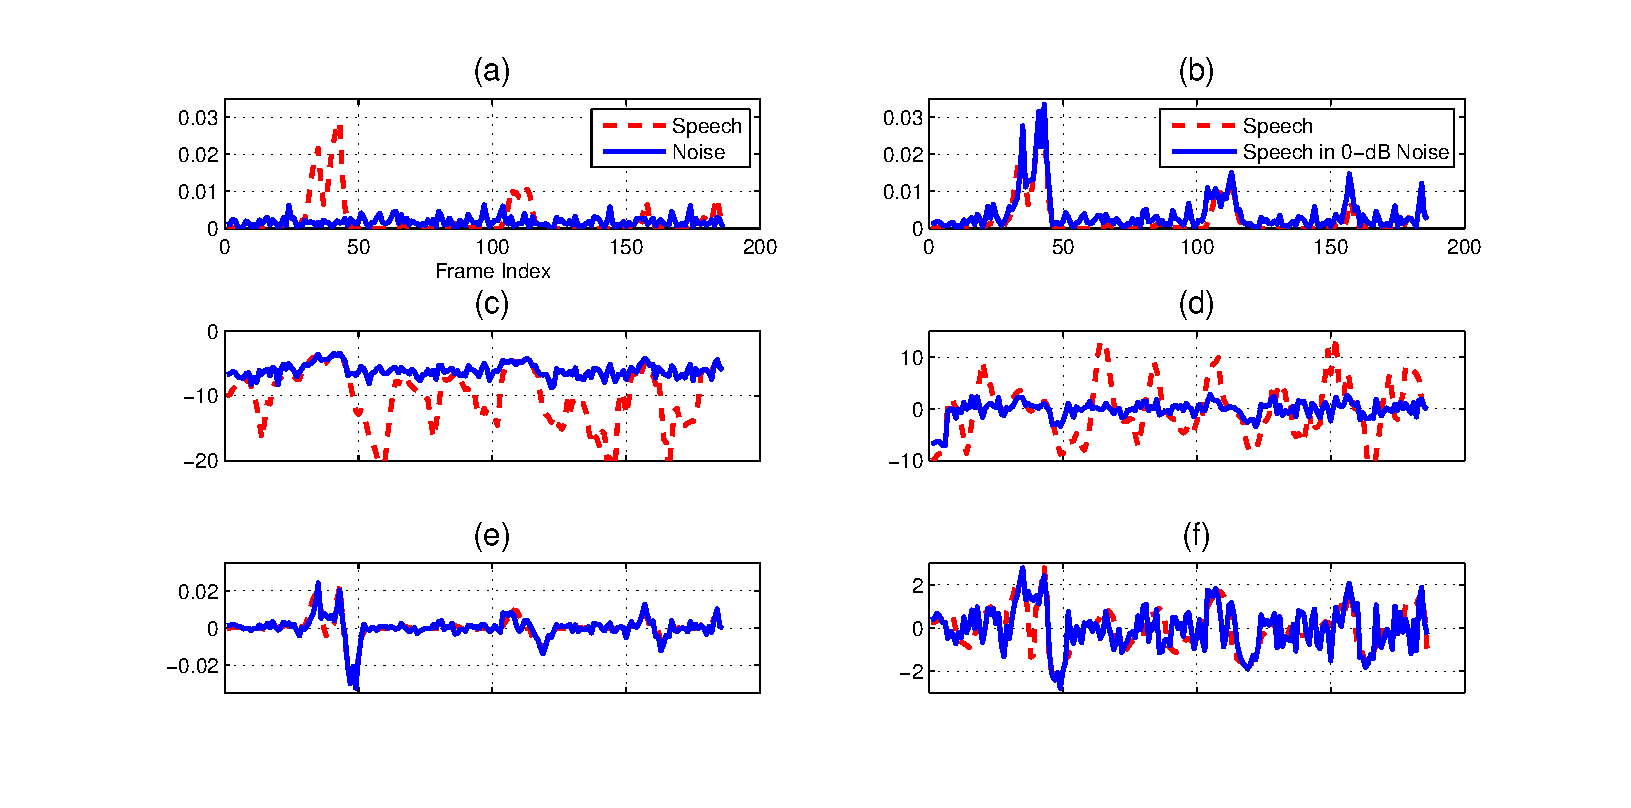
\includegraphics[width=1\textwidth]{deltaspectra_cepstra2.eps}
\caption{(a) Short-time power plot of a mel channel (center frequency 1000 Hz) for a speech and a ``real-world'' noise
segment using 10-ms frames.   (b) Short-time power for clean speech as in (a) and speech in  0-dB ``real-world'' noise from (a).
(c) Logarithmic power plot for clean speech and noisy speech in (b). (d) Temporal difference operation over
the signals in (c). (e) Temporal difference over the signals in (b). (f) Gaussianization operation over the signals in (e).}
\label{Fig:delta-samsung}
\end{figure*}

\begin{equation}\label{Eq:delta_features}
D[n] = C[n+m] - C[n-m]
\end{equation}
where $n$ is the index of the analysis frames and in practice $m$ is approximately  2 or 3. Similarly, double-delta cepstral features are defined in terms of a subsequent delta-operation on the delta-cepstral features. Fig.~\ref{Fig:MFCC_Delta} plots the word error rate (WER) for speech recognition in the presence of white noise for the  DARPA Resource Management (RM) database, following experimental procedures described in Sec.~\ref{sec:experiments}. We note that the addition of delta-cepstral features to the static 13-dimensional MFCC features strongly improves speech recognition accuracy, and a further (smaller) improvement is provided by the addition of  double-delta cepstral. For these reasons some form of delta and double-delta cepstral features are part of nearly   all   speech recognition systems.  It can be seen that the improvement provided by delta features gradually
diminishes with lower SNR.  We also note that from Eq. \eqref{Eq:delta_features}, it can be easily shown that $E[D[n]C[n]] = 0$, where $E[.]$ is expectation operator, so the delta-features are uncorrelated with the static features and help the frame independence assumption in the HMM in ASR.


While the addition of delta-cepstral coefficients (DCC) to MFCC coefficients does indeed improve ASR recognition accuracy, they do not provide good robustness in noise and reverberation.    The reasons for this can be understood in graphical form by consideration of Fig.~\ref{Fig:delta-samsung}, which depicts various manipulations of the short-time power of clean speech, and speech in  ``real-world'' noise at 0-dB SNR (with noise recorded naturally from locations such as a market, a food court, the street, and a bus stop). Fig.~\ref{Fig:delta-samsung}(a) plots the short-time power for a particular speech segment, and for the corresponding noise segment. We note that the speech  signal power exhibits a very high dynamic range, while the noise spectral power is much more  static than the speech power. Fig.~\ref{Fig:delta-samsung}(b) plots the short-time power for clean speech and speech plus noise at 0 dB noise using the noise from Fig.~\ref{Fig:delta-samsung}(a). Unsurprisingly,  the peaks of Fig.~\ref{Fig:delta-samsung}(b) remain relatively intact, while the  ``valleys'' are filled by the noise. The corresponding log power values  are shown in Fig.~\ref{Fig:delta-samsung}(c), and they are a step in the extraction of MFCC coefficients, as seen in
Fig.~\ref{Fig:blockdiag}(a).  Due to the compressive nature of the log nonlinearity, the spectral peaks are approximately the same for the clean and noisy speech but the remaining frames exhibit a high degree of mismatch. Since noise fills the the   valleys of the curves, and the noise is relatively stationary, the noisy log-spectral contour exhibits a sharply reduced dynamic range in comparison to the corresponding clean log-spectral contour. Finally, plotting the corresponding  delta-cepstral
features in Fig.~\ref{Fig:delta-samsung}(d) we note that the delta features still exhibit a high degree of mismatch between clean and noisy conditions. The delta-spectral features proposed in the next section both retain the contextual properties of delta-cepstral features and   are   robust to noise and reverberation as well.

%\vspace{-.5 cm}
\section{Delta-Spectral Cepstral Coefficients}\label{sec:DSCC}
We now discuss the delta-spectral cepstral coefficients for ASR. These features are motivated by the non-stationarity of  speech signals that had been observed in Fig.~\ref{Fig:delta-samsung}(a) where it is easily observed in that figure that the short-time power of speech varies much more rapidly than the short-time power of noise.    The vast differences between the rate of change of  power for of speech and noise are likely to be one of the many cues that  human ears can use to ignore the relatively stationary noise signals and focus on  the rapidly-changing power of speech signals.

The proposed  delta-spectral ceptral coefficient
(DSCC) features are described in block diagram form in Fig.~\ref{Fig:blockdiag}(b). Our objective is to combine the  speech contextual information   captured by the DCC features in Fig.~\ref{Fig:blockdiag}(a) with a greater degree of  robustness to additive noise. As can be seen, the major changes are that the initial time-differencing operation is now earlier in the processing and a new Gaussianization stage is added. Specifically, performing the delta operation described by Eq.~\eqref{Eq:delta_features}    in the spectral domain will enhance the fast changing speech components, and suppress the slowly-changing noisy components.  Fig.~\ref{Fig:delta-samsung}(e) plots the outcome  of the delta operation in the spectral domain on the power contours in Fig.~\ref{Fig:delta-samsung}(b).  The advantage of the delta-spectral approach is clear by comparison of the similarity of the  curves representing clean and noisy speech in Fig.~\ref{Fig:delta-samsung}(e) (which were obtained by applying the delta operation in the spectral domain) to the corresponding curves in Fig.~\ref{Fig:delta-samsung}(d) (which were obtained by applying the delta operation in the cepstral domain). However,  the delta-spectral features
in their current form are unsuitable for speech recognition applications because the raw delta-spectral cepstral features are highly non-Gaussian, as is seen in Fig.~\ref{Fig:Gaussianization}.  To adapt the delta-spectral features for  speech recognition, we apply histogram  normalization to the delta-spectral features to give them a Gaussian distribution, as shown in   Fig.~\ref{Fig:Gaussianization}(b). This Gaussianization nonlinearity is applied on  an utterance-by-utterance basis. Fig.~\ref{Fig:delta-samsung}(f) plots the ``Gaussianized'' delta-spectral features, which are   reduced by the DCT operation as in Fig.~\ref{Fig:blockdiag}(b) to a 13-dimensional vector of delta-spectral cepstral coefficients (DSCC). Double-delta features are then derived from the delta-spectral features in the cepstral domain.


\section{DSCC Feature Analysis}\label{sec:analysis}
In this section we provide a more formal analysis of the SNR improvement in white noise   using the DSCC features.    Assuming that the noise is a white   Gaussian   sequence sample distribution $w_i$ of the form
 $\mathcal{N}(0,\sigma^2)$, the power $P$ in an independently-observed set of $N$ samples is
 $P = \frac{1}{N}\sum_{i=1}^Nw_i^2$. $P$ follows a chi-square distribution with $N$ degrees of freedom (DOF), which becomes   approximately Gaussian for large $N$. Under the Gaussian   assumption
  for $P$, it can be shown that
\begin{eqnarray*}
E[P] &=& \frac{1}{N}E[\sum_{i=1}^Nw_i^2] = \sigma^2\\
\end{eqnarray*}
\begin{eqnarray*}
Var[P] &=& E[P^2] - E[P]^2 = \frac{E\big[\sum_{i,j}{w_i^2 w_j^2}\big]}{N^2} - \sigma^4\\
%&= \frac{1}{N^2}\left(\sum_{i}E[{x_i^4}] + \displaystyle\sum_{i,j,i\neq j}E[x_i^2 x_i^2]\end\right) - \sigma^4 = \frac{2\sigma^4}{N}
&=& \frac{1}{N^2}\Bigl(\sum_{i}E[{w_i^4}] + \displaystyle\sum_{i,j,i\neq j}E[w_i^2 w_i^2]\Bigr) - \sigma^4 = \frac{2\sigma^4}{N}
\end{eqnarray*}
Thus, $P$ is approximately distributed as $\emph{N}(\sigma^2,\frac{2\sigma^4}{N})$.  The    DC power associated with $P$ is  the square of the mean, $\sigma^4$, while the AC power is the variance $\frac{2\sigma^4}{N}$.    DSCC processing  removes the DC power, and we can express the impact of this effect using the ratio  \begin{eqnarray*}
\mbox{Noise suppression} &\approx& -10\,\log_{10}\Bigl(\frac{Pow_{AC}}{Pow_{AC}+Pow_{DC}}\Bigl)\\
                          & =&\;\;\;10\,\log_{10}\bigl(1+N/2\bigl)
\end{eqnarray*}
We use a speech analysis window duration of 25 ms, so the number of samples in the window duration becomes $N=400$
with a   sampling frequency of 16,000 Hz, and for $N=400$, the consequent  white noise suppression is 23.03 dB.
Thus, the maximum possible benefit with DSCC processing is a 23-dB SNR noise suppression for the white noise case.
\begin{table}[h]
\label{T:noise_suppress}
\centering
\begin{tabular}[h]{|c|c|c|c|c|}
\hline
Noise Type & White & Real-World  & Music\\
\hline
Predicted noise suppression & 23 &12 &3.5\\
\hline
SNR threshold-shift in ASR & 8.3 & 7.5 &5\\
\hline
\end{tabular}
\caption{Predicted noise suppression and observed SNR threshold-shift in an ASR experiment for different noise conditions (in dB)}
\end{table}

In Table~\ref{T:noise_suppress}, we experimentally derive the degree of noise suppression for different noise conditions based on the percentage of total power that is DC power, as above. As expected,
the noise-suppression so obtained is greater for relatively stationary noises such as  white noise and the ``real-noise''   conditions than for background.
We also present the experimentally-observed  shift in effective SNR that will discussed below in conjunction with a speech-recognition task (\emph{cf.} Fig.~\ref{Fig:WER_plots_delta}).
While the observed shifts SNR   shifts are not equal to the calculations above for many reasons, (including suppression of both speech and noise at other frequencies imposed by the DSCC algorithm and subsequent nonlinearities in processing), the trends of the dependencies are similar, suggesting that closer study of the impact of processing on the modulation spectra can provide insight into the extent to which DSCC and similar processing can reduce the impact of various types of noise.

\begin{figure}[h]
\centering
{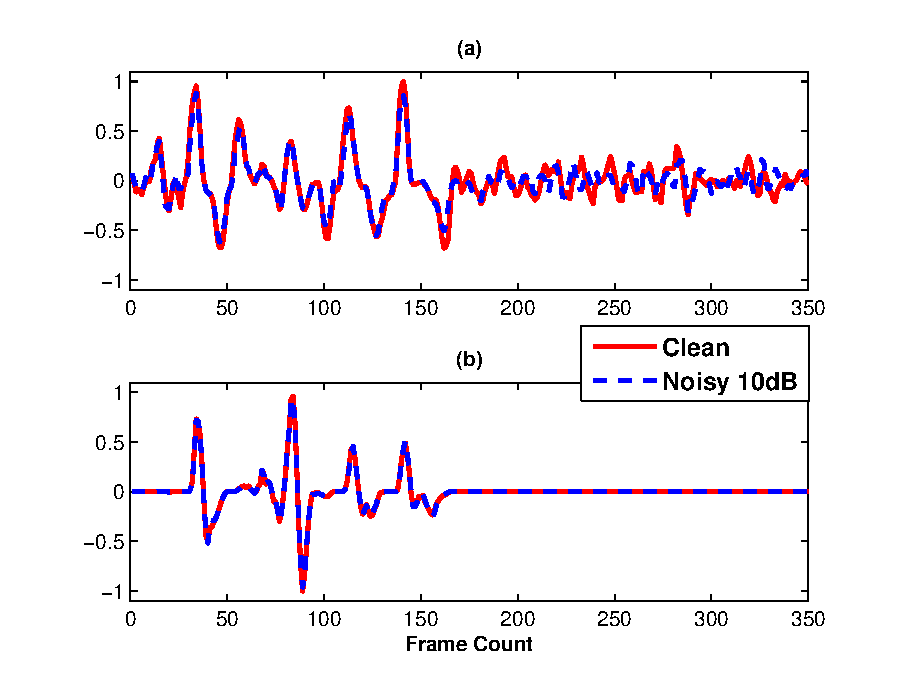
\includegraphics[width=0.47\textwidth]{Mel8-Delta.eps}}
\caption{\it Arbitration for client and service ASR resuls.}
\label{Fig:Arbitration}
\end{figure}



\section{Experimental results}\label{sec:experiments}

We describe in this section experimental results comparing DSCC features to conventional MFCC/DCC and other features using  degraded speech from  the DARPA Resource Management (RM) database, which consists  of  1600 training utterances and 600 test utterances. Data  were obtained by digitally adding the various noises described above to the speech signal. We also evaluated the features in reverberant environments, which were simulated by   convolving the speech from the  RM database with simulated room impulse responses using the (RIR) software package\footnote{\url{http://2pi.us/rir.html}} \cite{LIFE10}. We used the Sphinx open source speech recognition   system\footnote{\url{http://cmusphinx.sourceforge.net/html/cmusphinx.php}} for   training and decoding, with   8 Gaussian Mixtures  and a bigram language model.

Fig.~\ref{Fig:WER_plots_delta},   compares the WER obtained using DCC, as in Fig.~\ref{Fig:blockdiag}(a), against DSCC, where temporal-differencing is performed in the  spectral domain,\footnote{The DSCC software is available at \url{http://www.cs.cmu.edu/ ~robust/archive/algorithms/DSCC_ICASSP2010/}.} as in Fig.~\ref{Fig:blockdiag}(b). These comparisons clearly demonstrate   the benefit of performing the time differencing in the spectral domain instead of in  the conventional cepstral domain. It can be seen that the delta-spectral features   substantial increases in robustness to noise as well as reverberation, increasing the effective SNR compared to by 5 to 8 dB at 50\% WER. The use of  DSCC features also provides a  30-45\% relative reduction in WER at reverberation times of $300-500$ ms.

Fig.~\ref{Fig:WER_plots} considers the combination of DSCC versus DCC features with MFCC, AFE \cite{AFE} and PNCC \cite{PNCC10}, it can be seen that the use of the DSCC features provides better recognition accuracy than what is obtained from DCC features for all noise and   reverberation conditions. The DSCC features not only strongly improve the baseline MFCC-DCC, they also improve the advanced systems in PNCC and AFE. Surprisingly we find that simply appending the 26-dim. DSCC features to the 13-dim. MFCC works as well as the conventional 39-dim. AFE features.

\section{Conclusions}\label{sec:conclusion}
In this study, we    propose   DSCC features that perform temporal differencing in the spectral rather than cepstral domain, and we observe that in comparison to conventional cepstral differencing,  the use of DSCC features improves the effective SNR by 4 to 8 dB for various types of additive noise and reduces the relative WER
by 20-30\% in reverberation.  We also find a good correspondence as a function of noise type between  the  extent to which the use of DSCC processing reduces the WER and noise and the fraction of noise power at DC.
\footnotesize

\bibliographystyle{IEEEbib}
\bibliography{strings}
\end{document}


%\begin{figure}[]
%\setlength{\unitlength}{.55cm}
%\footnotesize
%\centering
%\begin{tabular}{c c}
%\subfigure[]{
%\centering
%\begin{picture}(4,16)
%\put(0, 17){\makebox(4,1){Input Speech}}
%\multiput(2,17)(0,-2){3}{\vector(0,-1){1}} % arrows on top
%\multiputlist(0,15)(0,-2)[lb]{{\framebox(4,1){Windowing}}, {\framebox(4,1){FFT}},{\framebox(4,1){Mel-Spectra}}}
%\put(2,11){\vector(0,-1){3}}
%\multiput(2,7)(0,-2){3}{\vector(0,-1){1}} % arrows on top
%\multiputlist(0,7)(0,-2)[lb]{{\framebox(4,1){Log}}, {\framebox(4,1){DCT}}, {\framebox(4,1){MVN}},{\framebox(4,1){\shortstack{+Delta\\+DDelta}}}}
%\put(0,-.25){\makebox(4,1){MFCC [39]}}
%\end{picture}}
%&
%\subfigure[]{
%\centering
%\begin{picture}(4,16)
%\put(0, 17){\makebox(4,1){Input Speech}}
%\multiput(2,17)(0,-2){8}{\vector(0,-1){1}} % arrows on top
%\multiputlist(0,15)(0,-2)[lb]{{\framebox(4,1){Windowing}}, {\framebox(4,1){FFT}}, {\framebox(4,1){Mel-Spectra}}, {\framebox(4,1){Delta-Spectra}}, {\framebox(4,1){\shortstack{Gaussianization\\Nonlinearity}}}, {\framebox(4,1){DCT}}, {\framebox(4,1){MVN}}, {\framebox(4,1){+Delta}}}
%\put(0,-.25){\makebox(4,1){DSCC [26]}}
%\end{picture}}
%\end{tabular}
%\caption{(a) 39-dimensional MFCC features, (b) 26-dimensional DSCC features.}
%\label{Fig:blockdiag}
%\end{figure}